\documentclass{article}
\usepackage{graphicx}
\usepackage{amsmath}
\usepackage{amssymb}
\usepackage{float}
\usepackage[margin=1in]{geometry}
\usepackage{listings}
\usepackage{xcolor}
\usepackage{verbatim}
\usepackage{tikz}
\usetikzlibrary{arrows.meta,positioning}
\graphicspath{{../}{./}}

\lstset{
  basicstyle=\ttfamily\footnotesize,
  breaklines=true,
  frame=single,
  numbers=left,
  numberstyle=\tiny,
  keywordstyle=\color{blue},
  commentstyle=\color{gray},
  showstringspaces=false
}

\title{IN4140 -- Assignment 4}
\author{John Ravndal}
\date{May 2026}

\begin{document}
\maketitle

\section{Introduction}

This report solves Task~1 (Control Theory) of Assignment~4 in IN4140. The task focuses on obtaining an independent joint model for Joint~2 of the simplified CrustCrawler, expressing the model in Laplace domain, deriving a closed-loop transfer function with a PD controller, and selecting gains that satisfy a specified natural frequency and damping requirement.

\section{Task 1 -- Control Theory (40\%)}

The goal is to obtain an independent joint equation for Joint~2, express it in Laplace form, derive the closed-loop transfer function with a PD controller, and compute controller gains that achieve a critically damped response with natural frequency $\omega_n=6$.

\subsection*{(a) Independent equation of motion for Joint 2}

From Assignment~3, the robot dynamics can be written on the standard form
\begin{equation}
    D(q)\ddot q + C(q,\dot q)\dot q + g(q) = \tau .
\end{equation}
For Joint~2, the second row gives
\begin{equation}
    \tau_2
    =
    d_{21}\ddot q_1
    +
    d_{22}\ddot q_2
    +
    d_{23}\ddot q_3
    +
    \sum_{i=1}^{3}\sum_{j=1}^{3} c_{ij2}\dot q_i \dot q_j
    +
    g_2(q).
    \label{eq:joint2_full}
\end{equation}

To make the equation independent, we assume that Joint~1 and Joint~3 are fixed while controlling Joint~2. Hence,
\begin{equation}
    \dot q_1 = \ddot q_1 = 0,
    \qquad
    \dot q_3 = \ddot q_3 = 0.
\end{equation}
This removes the acceleration coupling terms from the other joints. It also removes the quadratic velocity terms involving $\dot q_1$ and $\dot q_3$. This is consistent with the assignment hint, since these quadratic terms describe effects induced by motion in the other joints.

The independent Joint~2 equation therefore becomes
\begin{equation}
    \tau_2 = J\ddot q_2 + g_2(q_2),
    \label{eq:joint2_independent}
\end{equation}
where
\begin{equation}
    J = d_{22}
\end{equation}
is the effective inertia seen by Joint~2.

From Assignment~3, the gravity term for Joint~2 was
\begin{equation}
    g_2(q)
    =
    \left(\frac{m_2}{2}+m_3\right)gL_2\cos q_2
    +
    \frac{m_3}{2}gL_3\cos(q_2+q_3).
\end{equation}
Since Joint~3 is fixed, we choose the fixed configuration $q_3=0$. Then
\[
    \cos(q_2+q_3)=\cos q_2,
\]
and the gravity term becomes
\begin{equation}
    g_2(q_2)
    =
    \left[
    \left(\frac{m_2}{2}+m_3\right)L_2
    +
    \frac{m_3}{2}L_3
    \right]g\cos q_2.
\end{equation}

Using the same center-of-mass approximation as in Assignment~3, the effective inertia is
\begin{equation}
    J
    =
    m_2\left(\frac{L_2}{2}\right)^2
    +
    m_3\left(L_2+\frac{L_3}{2}\right)^2.
\end{equation}

Thus, the independent equation of motion for Joint~2 is
\begin{equation}
    \boxed{
    \tau_2
    =
    \left[
    m_2\left(\frac{L_2}{2}\right)^2
    +
    m_3\left(L_2+\frac{L_3}{2}\right)^2
    \right]\ddot q_2
    +
    \left[
    \left(\frac{m_2}{2}+m_3\right)L_2
    +
    \frac{m_3}{2}L_3
    \right]g\cos q_2
    }.
\end{equation}

For the remaining tasks, we write
\[
    \theta := q_2,
    \qquad
    u := \tau_2,
\]
so the independent model can be written as
\begin{equation}
    u(t) = J\ddot\theta(t) + G\cos\theta(t),
\end{equation}
where
\[
    G =
    \left[
    \left(\frac{m_2}{2}+m_3\right)L_2
    +
    \frac{m_3}{2}L_3
    \right]g.
\]

\subsection*{(b) Laplace transform and identification of $J$, $B$, and $D$}

The generic independent joint model given in the assignment is
\begin{equation}
    u(t) = J\ddot{\theta}(t) + B\dot{\theta}(t) + D(t),
    \label{eq:generic_joint_time}
\end{equation}
where $J$ is the effective inertia, $B$ is viscous damping, and $D(t)$ represents disturbance terms. In this context, the disturbance includes gravity and any effects that are not included in the simple linear joint model.

Taking the Laplace transform of~\eqref{eq:generic_joint_time}, and assuming zero initial conditions, gives
\begin{equation}
    U(s) = Js^2\Theta(s) + Bs\Theta(s) + D(s).
\end{equation}
This can be written as
\begin{equation}
    U(s) = (Js^2 + Bs)\Theta(s) + D(s).
    \label{eq:generic_joint_laplace}
\end{equation}

Equivalently, solving for the joint angle gives
\begin{equation}
    \Theta(s)
    =
    \frac{U(s)-D(s)}{Js^2+Bs}.
    \label{eq:theta_laplace}
\end{equation}
Thus, if the disturbance is ignored when deriving the basic plant model, the transfer function from input torque to joint angle is
\begin{equation}
    G(s)
    =
    \frac{\Theta(s)}{U(s)}
    =
    \frac{1}{Js^2+Bs}.
    \label{eq:plant_transfer_function}
\end{equation}

From Task~1a, the independent Joint~2 model was
\begin{equation}
    u(t) = J\ddot{\theta}(t) + G\cos\theta(t),
\end{equation}
where
\begin{equation}
    J
    =
    m_2\left(\frac{L_2}{2}\right)^2
    +
    m_3\left(L_2+\frac{L_3}{2}\right)^2,
\end{equation}
and
\begin{equation}
    G
    =
    \left[
    \left(\frac{m_2}{2}+m_3\right)L_2
    +
    \frac{m_3}{2}L_3
    \right]g.
\end{equation}

Comparing this with the generic model in~\eqref{eq:generic_joint_time}, we identify
\begin{equation}
    \boxed{
    J
    =
    m_2\left(\frac{L_2}{2}\right)^2
    +
    m_3\left(L_2+\frac{L_3}{2}\right)^2
    }
\end{equation}
as the effective inertia of Joint~2. Since no viscous damping term was derived in Assignment~3, we set
\begin{equation}
    \boxed{B = 0}.
\end{equation}
Finally, the disturbance term is the gravity torque
\begin{equation}
    \boxed{
    D(t) = G\cos\theta(t)
    =
    \left[
    \left(\frac{m_2}{2}+m_3\right)L_2
    +
    \frac{m_3}{2}L_3
    \right]g\cos\theta(t)
    }.
\end{equation}

Therefore, for the model derived in Task~1a, the Laplace-domain equation becomes
\begin{equation}
    U(s) = Js^2\Theta(s) + D(s),
\end{equation}
or
\begin{equation}
    \Theta(s) = \frac{U(s)-D(s)}{Js^2}.
\end{equation}

\subsection*{(c) Closed-loop block diagram and transfer function with PD control}

From Task~1b, the independent Joint~2 plant model in Laplace domain is
\begin{equation}
    \Theta(s) = \frac{U(s)-D(s)}{Js^2+Bs}.
    \label{eq:plant_disturbance}
\end{equation}
This means that the plant from control input torque to joint angle is
\begin{equation}
    G(s) = \frac{\Theta(s)}{U(s)} = \frac{1}{Js^2+Bs},
    \label{eq:plant_G}
\end{equation}
when the disturbance term is ignored for the reference-to-output transfer function.

Figure~\ref{fig:plant_model} shows the independent joint plant model. The disturbance $D(s)$ is subtracted from the control input $U(s)$ before the signal enters the plant.

\begin{figure}[H]
    \centering
    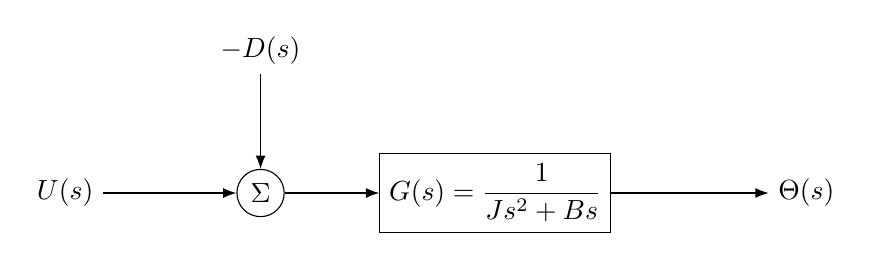
\begin{tikzpicture}[
        block/.style={draw, rectangle, minimum height=1cm, minimum width=2.4cm},
        sum/.style={draw, circle, inner sep=1pt, minimum size=6mm},
        >=Latex
    ]
        \node[sum] (sum) {};
        \node[block, right=1.2cm of sum] (plant) {$G(s)=\dfrac{1}{Js^2+Bs}$};
        \draw[->] (sum) -- (plant);
        \draw[->] (plant.east) -- ++(2.0cm,0) node[right] {$\Theta(s)$};
        \draw[->] ++(-2.0cm,0) node[left] {$U(s)$} -- (sum);
        \draw[->] (sum.north) ++(0,1.2cm) node[above] {$-D(s)$} -- (sum.north);
        \node at (sum) {$\Sigma$};
    \end{tikzpicture}
    \caption{Independent Joint~2 plant model with disturbance.}
    \label{fig:plant_model}
\end{figure}

To control the joint position, we use unity negative feedback. The error signal is defined as
\begin{equation}
    E(s) = \Theta_d(s) - \Theta(s),
\end{equation}
where $\Theta_d(s)$ is the desired joint angle and $\Theta(s)$ is the measured joint angle.

A PD controller is used:
\begin{equation}
    C(s) = K_P + K_Ds.
    \label{eq:pd_controller}
\end{equation}
The controller output is therefore
\begin{equation}
    U(s) = C(s)E(s)
    =
    (K_P + K_Ds)\left(\Theta_d(s)-\Theta(s)\right).
\end{equation}

The complete closed-loop system is shown in Figure~\ref{fig:closed_loop_pd}. The output angle $\Theta(s)$ is fed back and subtracted from the desired angle $\Theta_d(s)$, producing the error signal used by the controller.

\begin{figure}[H]
    \centering
    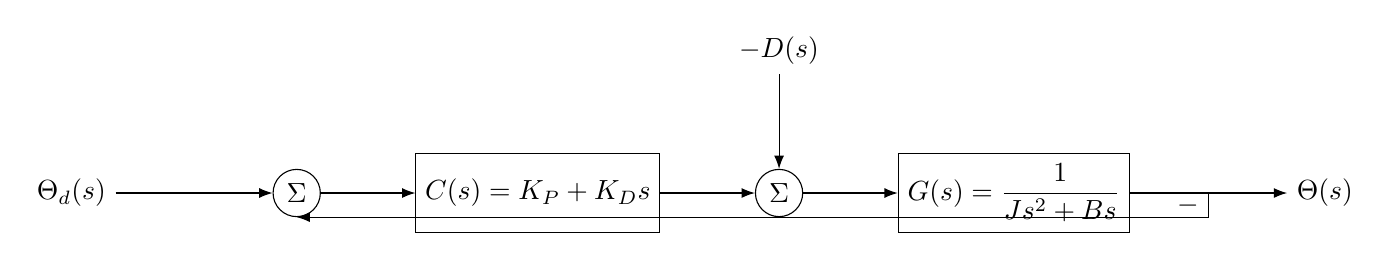
\begin{tikzpicture}[
        block/.style={draw, rectangle, minimum height=1cm, minimum width=2.6cm},
        sum/.style={draw, circle, inner sep=1pt, minimum size=6mm},
        >=Latex
    ]
        \node[sum] (sum) {};
        \node[block, right=1.2cm of sum] (ctrl) {$C(s)=K_P+K_Ds$};
        \node[sum, right=1.2cm of ctrl] (sum2) {};
        \node[block, right=1.2cm of sum2] (plant) {$G(s)=\dfrac{1}{Js^2+Bs}$};

        \draw[->] (sum) -- (ctrl);
        \draw[->] (ctrl) -- (sum2);
        \draw[->] (sum2) -- (plant);
        \draw[->] (plant.east) -- ++(2.0cm,0) node[right] {$\Theta(s)$};

        \draw[->] ++(-2.3cm,0) node[left] {$\Theta_d(s)$} -- (sum);
        \draw[->] (plant.east) ++(1.0cm,0) |- (sum.south) node[pos=0.25, left] {$-$};

        \draw[->] (sum2.north) ++(0,1.2cm) node[above] {$-D(s)$} -- (sum2.north);
        \node at (sum) {$\Sigma$};
        \node at (sum2) {$\Sigma$};
    \end{tikzpicture}
    \caption{Closed-loop Joint~2 control system with PD controller.}
    \label{fig:closed_loop_pd}
\end{figure}

For the transfer function from desired angle $\Theta_d(s)$ to actual angle $\Theta(s)$, we set the disturbance $D(s)=0$. Then the closed-loop transfer function becomes
\begin{equation}
    \frac{\Theta(s)}{\Theta_d(s)}
    =
    \frac{C(s)G(s)}{1+C(s)G(s)}.
\end{equation}
Substituting
\[
    C(s)=K_P+K_Ds,
    \qquad
    G(s)=\frac{1}{Js^2+Bs},
\]
gives
\begin{equation}
    \frac{\Theta(s)}{\Theta_d(s)}
    =
    \frac{\frac{K_P+K_Ds}{Js^2+Bs}}
    {1+\frac{K_P+K_Ds}{Js^2+Bs}}.
\end{equation}
Multiplying numerator and denominator by $Js^2+Bs$ gives
\begin{equation}
    \boxed{
    \frac{\Theta(s)}{\Theta_d(s)}
    =
    \frac{K_Ds+K_P}
    {Js^2+(B+K_D)s+K_P}
    }.
    \label{eq:closed_loop_tf}
\end{equation}

This is the closed-loop transfer function for the independent Joint~2 model with a PD controller.
\subsection*{(d) Gains for $\omega_n = 6$ and critical damping}

From Task~1c, the closed-loop transfer function with a PD controller was
\begin{equation}
    \frac{\Theta(s)}{\Theta_d(s)}
    =
    \frac{K_Ds+K_P}
    {Js^2+(B+K_D)s+K_P}.
\end{equation}
The characteristic polynomial is therefore the denominator
\begin{equation}
    Js^2+(B+K_D)s+K_P.
\end{equation}
Dividing by $J$ gives the normalized characteristic polynomial
\begin{equation}
    s^2 + \frac{B+K_D}{J}s + \frac{K_P}{J}.
    \label{eq:charpoly_norm}
\end{equation}

A standard second-order system has characteristic polynomial
\begin{equation}
    s^2 + 2\zeta\omega_n s + \omega_n^2.
    \label{eq:second_order}
\end{equation}
The assignment specifies a natural frequency
\[
    \omega_n = 6
\]
and a critically damped system, which means
\[
    \zeta = 1.
\]
Matching coefficients between~\eqref{eq:charpoly_norm} and~\eqref{eq:second_order} gives
\begin{align}
    \frac{B+K_D}{J} &= 2\zeta\omega_n = 12, \\
    \frac{K_P}{J} &= \omega_n^2 = 36.
\end{align}
Therefore,
\begin{equation}
    K_P = 36J,
    \qquad
    K_D = 12J - B.
    \label{eq:kp_kd_general}
\end{equation}

From Task~1b, no viscous damping term was included in the derived model, so
\[
    B = 0.
\]
Using the effective inertia from Task~1a,
\begin{equation}
    J
    =
    m_2\left(\frac{L_2}{2}\right)^2
    +
    m_3\left(L_2+\frac{L_3}{2}\right)^2,
\end{equation}
the gains become
\begin{equation}
    \boxed{
    K_P
    =
    36
    \left[
    m_2\left(\frac{L_2}{2}\right)^2
    +
    m_3\left(L_2+\frac{L_3}{2}\right)^2
    \right]
    }
\end{equation}
and
\begin{equation}
    \boxed{
    K_D
    =
    12
    \left[
    m_2\left(\frac{L_2}{2}\right)^2
    +
    m_3\left(L_2+\frac{L_3}{2}\right)^2
    \right]
    }.
\end{equation}

Using the numerical values
\[
    m_2 = 0.2724\,\mathrm{kg},
    \qquad
    m_3 = 0.1406\,\mathrm{kg},
\]
\[
    L_2 = 0.2221\,\mathrm{m},
    \qquad
    L_3 = 0.1362\,\mathrm{m},
\]
we get
\begin{equation}
    J
    =
    0.2724\left(\frac{0.2221}{2}\right)^2
    +
    0.1406\left(0.2221+\frac{0.1362}{2}\right)^2
    \approx 0.01520.
\end{equation}
Therefore,
\begin{equation}
    \boxed{
    K_P \approx 0.547
    }
\end{equation}
and
\begin{equation}
    \boxed{
    K_D \approx 0.182
    }.
\end{equation}

\section{Task 3 -- Simulation I (35\%)}

In this task we control the position of Joint~2 in the CrustCrawler simulation using the provided ROS2 controller framework. The controller is implemented in \texttt{pid\_assignment/src/pid\_assignment/pid.py} and is exercised through the ROS2 node in \texttt{pid\_assignment/src/pid\_assignment/node.py}, which publishes effort commands to Joint~2 and publishes controller state for logging/plotting.

\subsection*{(a) PD-controller implementation and response}

The PD control law was implemented as
\begin{equation}
    u(t) = K_P\big(\theta_d(t)-\theta(t)\big) + K_D\frac{d}{dt}\big(\theta_d(t)-\theta(t)\big).
\end{equation}
In the implementation, the derivative action is applied on the measured joint velocity (derivative-on-measurement) to avoid a large derivative kick when the set-point changes:
\begin{equation}
    u(t) = K_P e(t) - K_D \dot{\theta}(t),
    \qquad
    e(t) = \theta_d(t)-\theta(t).
\end{equation}

Figure~\ref{fig:task3a_pd_step} shows the simulated step response for a set-point change to $\theta_d = 0.5$~rad using a PD controller (parameters in the plot: $K_P=5.0$, $K_D=1.0$, $K_I=0$). The plotted signals are the set-point, process value (joint position), and error.

\begin{figure}[H]
    \centering
    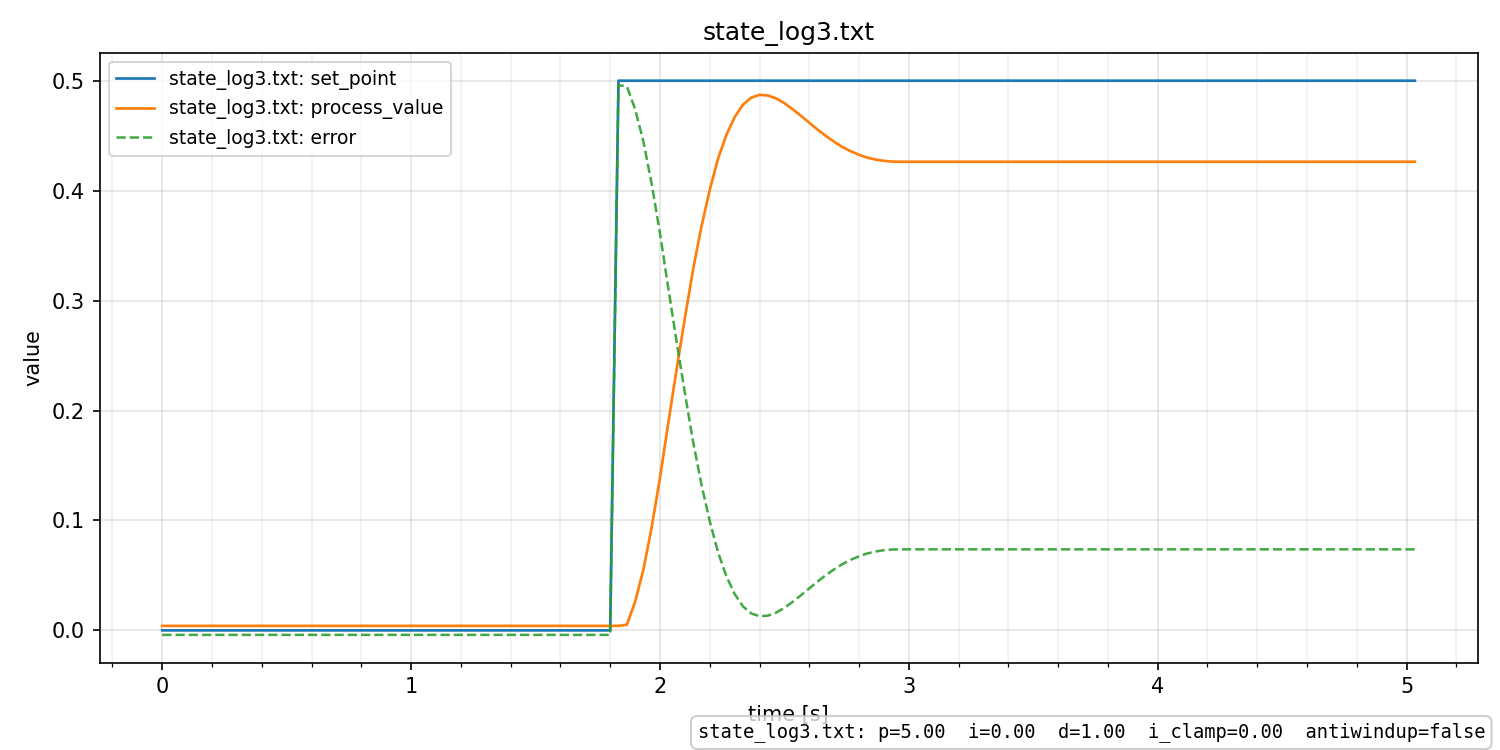
\includegraphics[width=0.95\textwidth]{state_plot_3a.png}
    \caption{Task 3a: Step response of Joint~2 with PD control.}
    \label{fig:task3a_pd_step}
\end{figure}

\paragraph{Settling time discussion.}
For an ideal second-order closed-loop system, the $5\%$ settling time is
\begin{equation}
    t_s = \frac{4}{\zeta \omega_n}.
\end{equation}
Using the design requirement from Task~1d of $\omega_n=6$ and critical damping $\zeta=1$ gives the nominal expectation
\[
    t_s \approx \frac{4}{6} \approx 0.67~\text{s}.
\]
The simulated response does not match this value exactly. The main reasons are that the simulation/plant differs from the simplified linear model used in Task~1: the joint dynamics are nonlinear (e.g., gravity torque depends on $\theta$), the controller runs in discrete time at about 30~Hz, and the PD controller does not reject constant disturbances perfectly (gravity/bias), which results in a nonzero steady-state error and changes the effective closed-loop behavior compared to the idealized second-order design.

\subsection*{(b) Controller tuning for lowest settling time without overshoot}

To reduce the settling time while avoiding overshoot, the controller gains were tuned experimentally by increasing $K_P$ to speed up the response, and then increasing $K_D$ to add damping until the response no longer exceeded the set-point. A step to $\theta_d=0.5$~rad was used as the test input.

After experimenting with several $(K_P,K_D)$ combinations, we found that the best performance (fast response without overshooting the set-point) was achieved with
\[
    K_P = 9.0,
    \qquad
    K_D = 2.0,
    \qquad
    K_I = 0.
\]
Figure~\ref{fig:task3b_tuned_pd} shows the resulting response. The position stays below the reference (no overshoot with respect to the set-point) and reaches its steady-state value quickly compared to the low-gain design from Task~1d.

\begin{figure}[H]
    \centering
    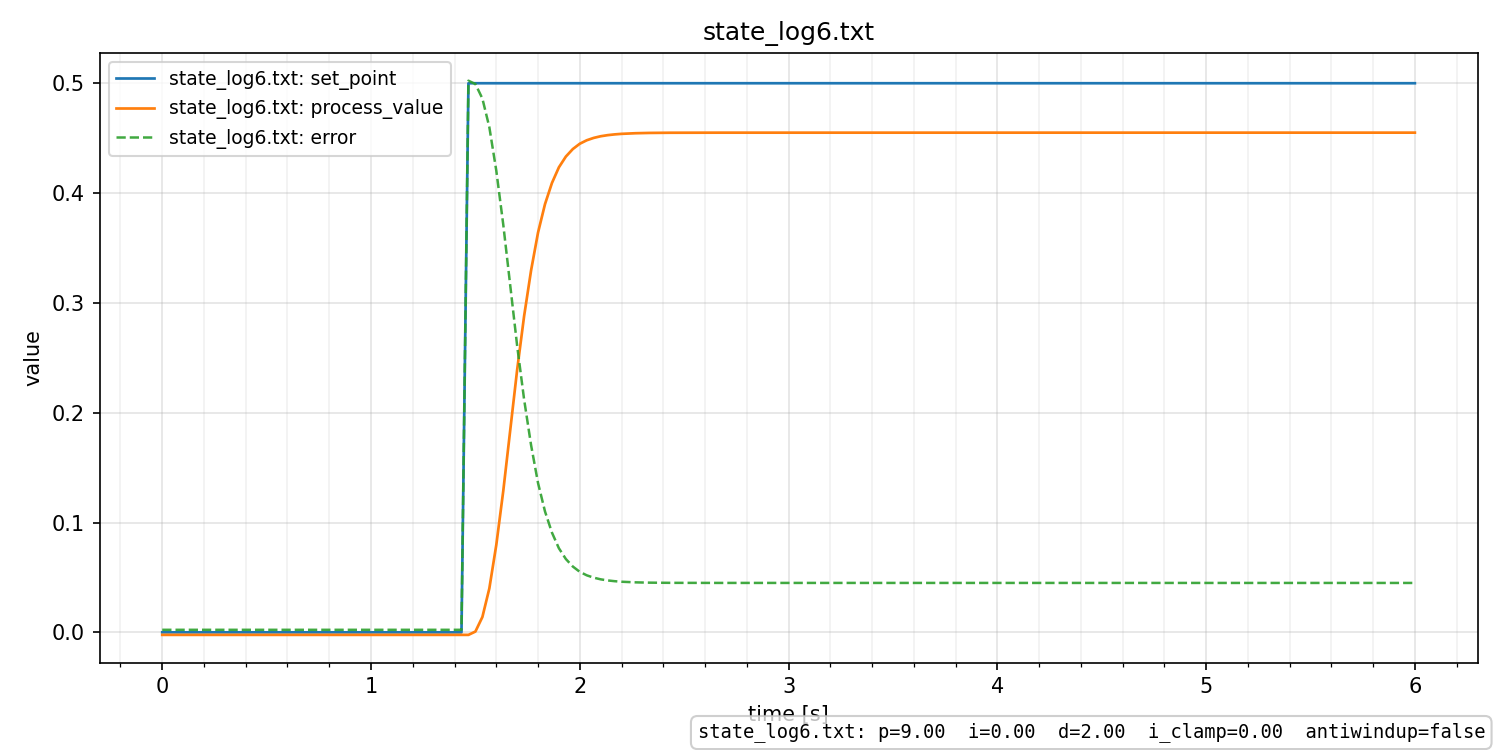
\includegraphics[width=0.95\textwidth]{state_plot_3b.png}
    \caption{Task 3b: Tuned PD response (set-point, position, error, and command).}
    \label{fig:task3b_tuned_pd}
\end{figure}

\paragraph{Steady-state error.}
From the steady-state value in Figure~\ref{fig:task3b_tuned_pd}, the joint position converges to approximately $\theta(\infty)\approx 0.455$~rad for a reference of $\theta_d=0.5$~rad. Thus the steady-state error is
\[
    e_{ss} = \theta_d - \theta(\infty) \approx 0.5 - 0.455 = 0.045~\text{rad}.
\]

\subsection*{(c) Is the steady-state error sufficiently small?}

With the tuned PD controller in Task~3b, we obtained a steady-state error of approximately $e_{ss}\approx 0.045$~rad ($\approx 2.6^\circ$) for a step to $\theta_d=0.5$~rad. This indicates that a PD controller alone does not fully reject the constant gravity/bias torque, and therefore leaves a nonzero offset.

To reduce this steady-state error, we extended the controller with an integral term and tuned a PID controller:
\[
    u(t) = K_P e(t) + K_I \int_0^t e(\tau)\,d\tau - K_D \dot{\theta}(t),
\]
where the integral action accumulates the persistent error and drives $e_{ss}\rightarrow 0$.

With $K_P=9.0$, $K_D=2.0$ and $K_I=0.8$, the response improved and the joint position converged close to the set-point (Figure~\ref{fig:task3c_pid}). However, we also observed that the error started oscillating again and peaked a second time roughly 30 seconds after the initial step, illustrating the trade-off: a larger $K_I$ reduces steady-state error, but can introduce slow oscillations/instability if tuned too aggressively.

\begin{figure}[H]
    \centering
    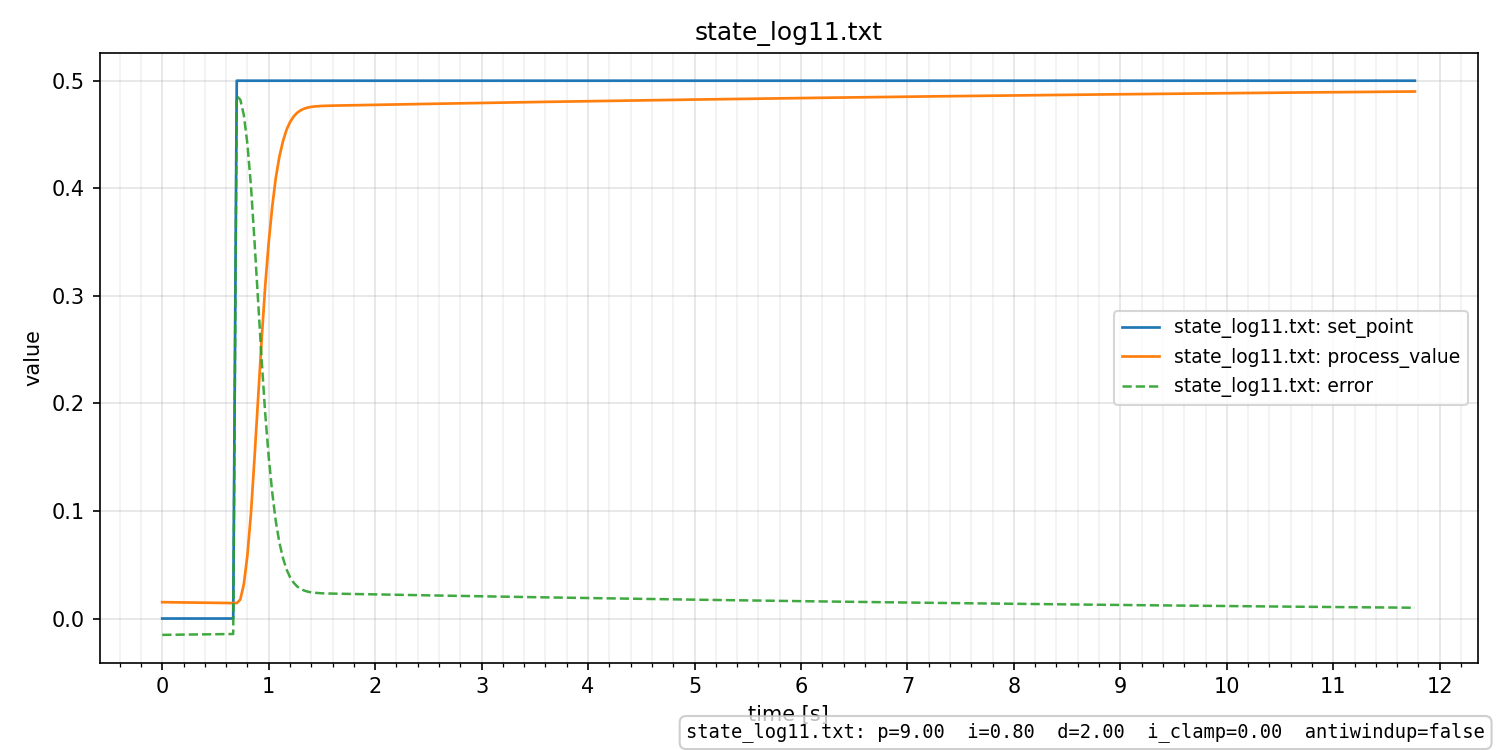
\includegraphics[width=0.95\textwidth]{state_plot_3c.png}
    \caption{Task 3c: Adding integral action ($K_I=0.8$) reduces steady-state error, but a slow oscillation reappears later (error peaks again after $\sim$30 s).}
    \label{fig:task3c_pid}
\end{figure}

\subsection*{(d) Expanded block diagram and transfer function}

In Task~3c, the steady-state error from the PD controller was reduced by adding an integral term. The controller was therefore changed from a PD controller to a PID controller:
\begin{equation}
    u(t)
    =
    K_P e(t)
    +
    K_I \int_0^t e(\tau)\,d\tau
    +
    K_D \dot e(t).
\end{equation}
In the implementation, the derivative term is applied on the measured joint velocity, but for the transfer function derivation we use the standard PID form.

Taking the Laplace transform gives
\begin{equation}
    U(s)
    =
    \left(
    K_P
    +
    \frac{K_I}{s}
    +
    K_Ds
    \right)E(s).
\end{equation}
Thus, the PID controller transfer function is
\begin{equation}
    C(s)
    =
    K_P
    +
    K_Ds
    +
    \frac{K_I}{s}.
\end{equation}

The plant model from Task~1 is still
\begin{equation}
    G(s)
    =
    \frac{1}{Js^2+Bs}.
\end{equation}
The expanded closed-loop block diagram is therefore the same as in Task~1c, except that the controller block is replaced by the PID controller
\[
    C(s)=K_P+K_Ds+\frac{K_I}{s}.
\]

\begin{figure}[H]
    \centering
    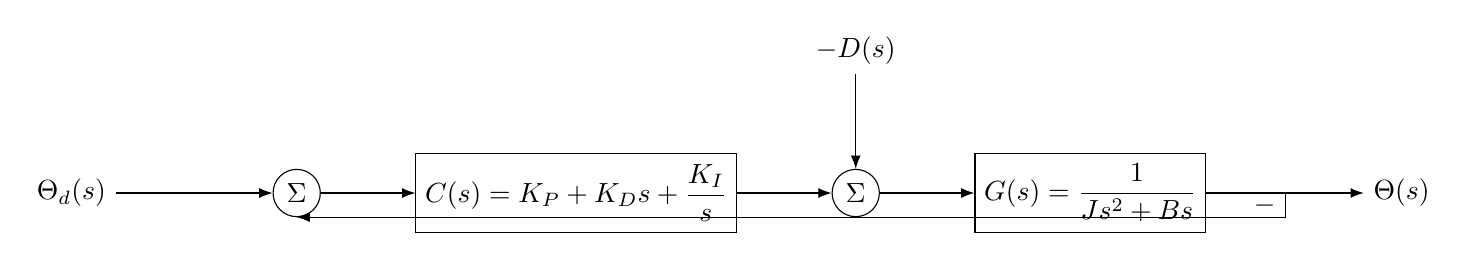
\begin{tikzpicture}[
        block/.style={draw, rectangle, minimum height=1cm, minimum width=2.9cm},
        sum/.style={draw, circle, inner sep=1pt, minimum size=6mm},
        >=Latex
    ]
        \node[sum] (sum) {};
        \node[block, right=1.2cm of sum] (ctrl) {$C(s)=K_P+K_Ds+\dfrac{K_I}{s}$};
        \node[sum, right=1.2cm of ctrl] (sum2) {};
        \node[block, right=1.2cm of sum2] (plant) {$G(s)=\dfrac{1}{Js^2+Bs}$};

        \draw[->] (sum) -- (ctrl);
        \draw[->] (ctrl) -- (sum2);
        \draw[->] (sum2) -- (plant);
        \draw[->] (plant.east) -- ++(2.0cm,0) node[right] {$\Theta(s)$};

        \draw[->] ++(-2.3cm,0) node[left] {$\Theta_d(s)$} -- (sum);
        \draw[->] (plant.east) ++(1.0cm,0) |- (sum.south) node[pos=0.25, left] {$-$};

        \draw[->] (sum2.north) ++(0,1.2cm) node[above] {$-D(s)$} -- (sum2.north);
        \node at (sum) {$\Sigma$};
        \node at (sum2) {$\Sigma$};
    \end{tikzpicture}
    \caption{Closed-loop Joint~2 control system with PID controller.}
    \label{fig:closed_loop_pid}
\end{figure}

For the reference-to-output transfer function, we set the disturbance $D(s)=0$. The closed-loop transfer function is
\begin{equation}
    \frac{\Theta(s)}{\Theta_d(s)}
    =
    \frac{C(s)G(s)}{1+C(s)G(s)}.
\end{equation}
Substituting
\[
    C(s)
    =
    K_P
    +
    K_Ds
    +
    \frac{K_I}{s}
    =
    \frac{K_Ds^2+K_Ps+K_I}{s}
\]
and
\[
    G(s)=\frac{1}{Js^2+Bs},
\]
gives
\begin{equation}
    \frac{\Theta(s)}{\Theta_d(s)}
    =
    \frac{K_Ds^2+K_Ps+K_I}
    {Js^3+(B+K_D)s^2+K_Ps+K_I}.
\end{equation}

Therefore, adding integral action changes the closed-loop system from a second-order system to a third-order system. The benefit is that the integral term accumulates persistent error and can remove steady-state error caused by constant disturbances such as gravity. The drawback is that too much integral gain can introduce slow oscillations or instability, which was observed in Task~3c.

\end{document}

